%%%%%%%%%%%%%%%%%%%%%%%%%%%%%%%%%%%%%%%%%
% Programming/Coding Assignment
% LaTeX Template
%
% This template has been downloaded from:
% http://www.latextemplates.com
%
% Original author:
% Ted Pavlic (http://www.tedpavlic.com)
%
% Note:
% The \lipsum[#] commands throughout this template generate dummy text
% to fill the template out. These commands should all be removed when 
% writing assignment content.
%
% This template uses a Perl script as an example snippet of code, most other
% languages are also usable. Configure them in the "CODE INCLUSION 
% CONFIGURATION" section.
%
%%%%%%%%%%%%%%%%%%%%%%%%%%%%%%%%%%%%%%%%%

%----------------------------------------------------------------------------------------
%	PACKAGES AND OTHER DOCUMENT CONFIGURATIONS
%----------------------------------------------------------------------------------------

\documentclass{article}

\usepackage{fancyhdr} % Required for custom headers
\usepackage{lastpage} % Required to determine the last page for the footer
\usepackage{extramarks} % Required for headers and footers
\usepackage[usenames,dvipsnames]{color} % Required for custom colors
\usepackage{graphicx} % Required to insert images
\usepackage{listings} % Required for insertion of code
\usepackage{courier} % Required for the courier font
\usepackage{lipsum} % Used for inserting dummy 'Lorem ipsum' text into the template
\usepackage{amsmath}
\usepackage{booktabs}
\usepackage{bigstrut}
\usepackage{float}
\usepackage{hyperref}
\usepackage{color}

\hypersetup{
    colorlinks   = true,    % Colours links instead of ugly boxes
    urlcolor     = red,    % Colour for external hyperlinks
    linkcolor    = red,    % Colour of internal links
    citecolor    = red      % Colour of citations
}
% Margins
\topmargin=-0.45in
\evensidemargin=0in
\oddsidemargin=0in
\textwidth=6.5in
\textheight=9.0in
\headsep=0.25in

\linespread{1.1} % Line spacing

% Set up the header and footer
\pagestyle{fancy}
\lhead{\hmwkAuthorName} % Top left header
\chead{\hmwkClass\ : \hmwkTitle} % Top center head
\rhead{\firstxmark} % Top right header
\lfoot{\lastxmark} % Bottom left footer
\cfoot{} % Bottom center footer
\rfoot{Page\ \thepage\ of\ \protect\pageref{LastPage}} % Bottom right footer
\renewcommand\headrulewidth{0.4pt} % Size of the header rule
\renewcommand\footrulewidth{0.4pt} % Size of the footer rule

\setlength\parindent{0pt} % Removes all indentation from paragraphs

%----------------------------------------------------------------------------------------
%	CODE INCLUSION CONFIGURATION
%----------------------------------------------------------------------------------------

\definecolor{MyDarkGreen}{rgb}{0.0,0.4,0.0} % This is the color used for comments
\lstloadlanguages{Perl} % Load Perl syntax for listings, for a list of other languages supported see: ftp://ftp.tex.ac.uk/tex-archive/macros/latex/contrib/listings/listings.pdf
\lstset{language=Perl, % Use Perl in this example
    frame=single, % Single frame around code
    basicstyle=\small\ttfamily, % Use small true type font
    keywordstyle=[1]\color{Blue}\bf, % Perl functions bold and blue
    keywordstyle=[2]\color{Purple}, % Perl function arguments purple
    keywordstyle=[3]\color{Blue}\underbar, % Custom functions underlined and blue
    identifierstyle=, % Nothing special about identifiers                                         
    commentstyle=\usefont{T1}{pcr}{m}{sl}\color{MyDarkGreen}\small, % Comments small dark green courier font
    stringstyle=\color{Purple}, % Strings are purple
    showstringspaces=false, % Don't put marks in string spaces
    tabsize=5, % 5 spaces per tab
    %
    % Put standard Perl functions not included in the default language here
    morekeywords={rand},
    %
    % Put Perl function parameters here
    morekeywords=[2]{on, off, interp},
    %
    % Put user defined functions here
    morekeywords=[3]{test},
    %
    morecomment=[l][\color{Blue}]{...}, % Line continuation (...) like blue comment
    numbers=left, % Line numbers on left
    firstnumber=1, % Line numbers start with line 1
    numberstyle=\tiny\color{Blue}, % Line numbers are blue and small
    stepnumber=5 % Line numbers go in steps of 5
}

% Creates a new command to include a perl script, the first parameter is the filename of the script (without .pl), the second parameter is the caption
\newcommand{\perlscript}[2]{
    \begin{itemize}
        \item[]\lstinputlisting[caption=#2,label=#1]{#1.py}
    \end{itemize}
}
\newcommand{\cppscript}[1]{
    \begin{itemize}
        \item[]\lstinputlisting[]{#1}
    \end{itemize}
}

%----------------------------------------------------------------------------------------
%	DOCUMENT STRUCTURE COMMANDS
%	Skip this unless you know what you're doing
%----------------------------------------------------------------------------------------

% Header and footer for when a page split occurs within a problem environment
\newcommand{\enterProblemHeader}[1]{
    \nobreak\extramarks{#1}{#1 continued on next page\ldots}\nobreak
    \nobreak\extramarks{#1 (continued)}{#1 continued on next page\ldots}\nobreak
}

% Header and footer for when a page split occurs between problem environments
\newcommand{\exitProblemHeader}[1]{
    \nobreak\extramarks{#1 (continued)}{#1 continued on next page\ldots}\nobreak
    \nobreak\extramarks{#1}{}\nobreak
}

%\setcounter{secnumdepth}{0} % Removes default section numbers
\newcounter{homeworkProblemCounter} % Creates a counter to keep track of the number of problems

\newcommand{\homeworkProblemName}{}
\newenvironment{homeworkProblem}[1][Problem \arabic{homeworkProblemCounter}]{ % Makes a new environment called homeworkProblem which takes 1 argument (custom name) but the default is "Problem #"
    \stepcounter{homeworkProblemCounter} % Increase counter for number of problems
    \renewcommand{\homeworkProblemName}{#1} % Assign \homeworkProblemName the name of the problem
    \section{\homeworkProblemName} % Make a section in the document with the custom problem count
    \enterProblemHeader{\homeworkProblemName} % Header and footer within the environment
    }{
    \exitProblemHeader{\homeworkProblemName} % Header and footer after the environment
}

\newcommand{\problemAnswer}[1]{ % Defines the problem answer command with the content as the only argument
\noindent\framebox[\columnwidth][c]{\begin{minipage}{0.98\columnwidth}#1\end{minipage}} % Makes the box around the problem answer and puts the content inside
}

\newcommand{\homeworkSectionName}{}
\newenvironment{homeworkSection}[1]{ % New environment for sections within homework problems, takes 1 argument - the name of the section
    \renewcommand{\homeworkSectionName}{#1} % Assign \homeworkSectionName to the name of the section from the environment argument
    \subsection{\homeworkSectionName} % Make a subsection with the custom name of the subsection
    \enterProblemHeader{\homeworkProblemName\ [\homeworkSectionName]} % Header and footer within the environment
    }{
    \enterProblemHeader{\homeworkProblemName} % Header and footer after the environment
}

%----------------------------------------------------------------------------------------
%	NAME AND CLASS SECTION
%----------------------------------------------------------------------------------------

\newcommand{\hmwkTitle}{homework 02} % Assignment title
\newcommand{\hmwkDueDate}{Tuesday,\ March\ 14,\ 2017} % Due date
\newcommand{\hmwkClass}{Numerical Analysis} % Course/class
\newcommand{\hmwkClassTime}{10:30am} % Class/lecture time
\newcommand{\hmwkClassInstructor}{Jones} % Teacher/lecturer
\newcommand{\hmwkAuthorName}{102061149 Fu-En Wang} % Your name

%----------------------------------------------------------------------------------------
%	TITLE PAGE
%----------------------------------------------------------------------------------------

\title{
    \vspace{2in}
    \textmd{\textbf{\hmwkClass:\ \hmwkTitle}}\\
    \normalsize\vspace{0.1in}\small{Due\ on\ \hmwkDueDate}\\
    \vspace{3in}
}

\author{\textbf{\hmwkAuthorName}}
\date{} % Insert date here if you want it to appear below your name

%----------------------------------------------------------------------------------------

\begin{document}

\maketitle
\newpage

\section{Introduction}
To solve such an equation:
\begin{gather}
    Ax = b
\end{gather}
where $A$ is $n \times n$ given nonsingular matrix and $b$ is a given vector, while $x$ is a vector to solve. Although Gaussion 
Elimination is an easy method for this problem, everytime when we adjust $b$, we have to re-calculate it again, which will be 
time-consuming. As a result, LU Decomposition provides a more flexible method to solve this problem.

\subsection{LU Decomposition}
Given a $n \times n$ matrix $A$, we can split it by:
\begin{gather}
    A = L \times U
\end{gather}
where $L$ is lower-triangular matrix and $U$ is upper-triangular matrix. And we can express $L$ and $U$ by this format:
\begin{gather}
    L = 
    \begin{bmatrix}
        1 & 0 & 0 \\
        u_{21}  & 1 & 0 \\
        u_{31}  & 0 & 1
    \end{bmatrix} 
\end{gather}
\begin{gather}
    U = 
    \begin{bmatrix}
        l_{11} & l_{12} & l_{13} \\
        0 & l_{22} & l_{23} \\
        0 & 0 & l_{33}
    \end{bmatrix} 
\end{gather}
So
\[
    A =
    \begin{bmatrix}
        1 & 0 & 0 \\
        u_{21}  & 1 & 0 \\
        u_{31}  & 0 & 1
    \end{bmatrix} 
    \times
    \begin{bmatrix}
        l_{11} & l_{12} & l_{13} \\
        0 & l_{22} & l_{23} \\
        0 & 0 & l_{33}
    \end{bmatrix} 
\]
After we find out $L$ and $U$, we can express problem by 
$$
    LUx = b
$$
Let $Y = Ux$, then
$$
    LY = b
$$
Y can be easily calculated, this is called \textbf{Forward Substitution}. After getting $Y$, the equation will be $Ux = Y$. $x$ can be
also easily calculated, this is called \textbf{Backward substitution}.

\subsection{Error Calculation}
Since the accuracy of our algorithm is quite important, I use sqare error to evaluate the performance:
\begin{gather}
    Error = \sqrt{\sum_{i=1}^{n}(b^{'}[i] - b[i])^2}
\end{gather}
where $b$ is the given vector and $b^{'}$ is the multiplication of $A$ and $x^{'}$ which is calculated by our algorithm.

\newpage

\section{C$++$ Implementation}
\subsection{LU Decomposition}
\cppscript{src/luFact.cpp}
\subsection{Forward Substitution}
\cppscript{src/fwdSubs.cpp}
\subsection{Backward Substitution}
\cppscript{src/bckSubs.cpp}

\section{Complexity}
\subsection{LU Decomposition}
In the outer double for-loop, we do $\frac{n(n+1)}{2}$ times of one additional for-loop, so this is a {\boldmath$O(n^3)$} problem.
\subsection{Forward/Backward substitution}
The double for-loop do $\frac{n(n+1)}{2}$ times of calculation, so this is a {\boldmath$O(n^2)$} problem.

\section{Discussion}
\subsection{Performance Evaluation}
In this project, I use 5 numbers to indicate the accuracy and efficiency of our method.
\begin{enumerate}
    \item \textbf{Error}(square error of the calculated result and answer)
    \item \textbf{Runtime}(total execution time of program)
    \item \textbf{LU}(total runtime consumed by LU Decomposition)
    \item \textbf{FWD}(total runtime consumed by Forward Substitution)
    \item \textbf{BCK}(total runtime consumed by Backward Substitution)
\end{enumerate}
Table \ref{tab:record} shows detailed result of m3 to m10 execution result.
% Table generated by Excel2LaTeX from sheet '工作表1'
\begin{table}[htbp]
  \centering
  \caption{Execution result of all matrix}
    \begin{tabular}{|c|c|c|c|c|c|c|c|c|}
    \hline
        & m3.dat & m4.dat & m5.dat & m6.dat & m7.dat & m8.dat & m9.dat & m10.dat \bigstrut\\
    \hline
    N   & 3   & 10  & 100 & 200 & 400 & 800 & 1600 & 3200 \bigstrut\\
    \hline
    Error & 0   & 1.11E-14 & 1.65E-10 & 2.52E-09 & 3.62E-08 & 6.30E-07 & 1.09E-05 & 0.000152939 \bigstrut\\
    \hline
    Runtime(s) & 0.005 & 0.004 & 0.007 & 0.026 & 0.162 & 1.137 & 9.343 & 67.129 \bigstrut\\
    \hline
    LU(s) & 0   & 2.00E-06 & 0.00187 & 0.015341 & 0.130141 & 1.02409 & 8.895 & 65.4746 \bigstrut\\
    \hline
    FWD(s) & 1.00E-06 & 1.00E-06 & 4.10E-05 & 0.000121 & 0.000467 & 0.002353 & 0.007206 & 0.028792 \bigstrut\\
    \hline
    BCK(s) & 0   & 1.00E-06 & 2.90E-05 & 0.00012 & 0.000479 & 0.001957 & 0.007655 & 0.03202 \bigstrut\\
    \hline
    \end{tabular}%
  \label{tab:record}%
\end{table}%

\begin{figure}[H]
    \centering
    \caption{Error vs $N^3$}
    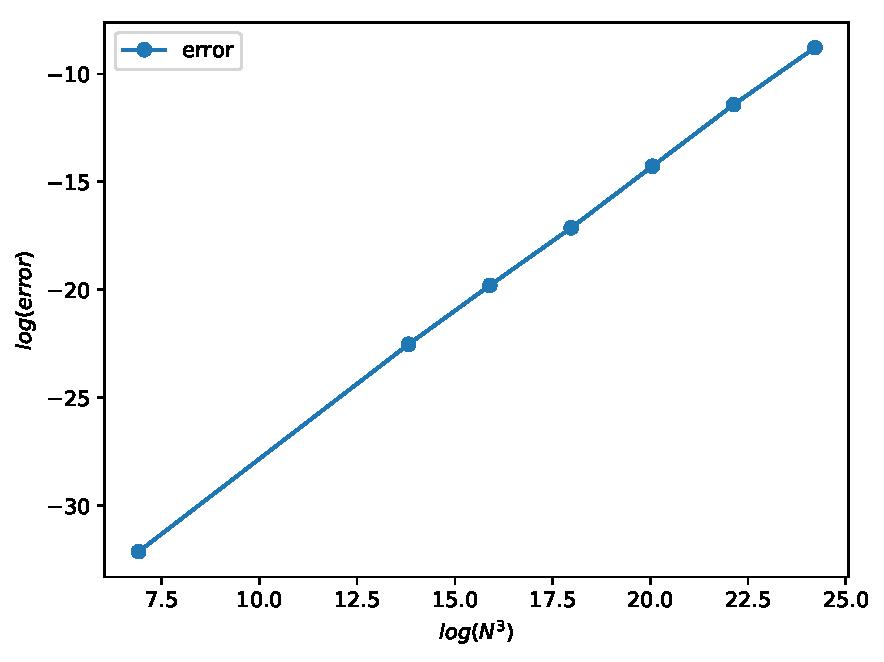
\includegraphics[width=0.65\textwidth]{src/error.pdf}
    \label{fig:error}
\end{figure}
\begin{figure}[H]
    \centering
    \caption{Runtime vs $N^3$}
    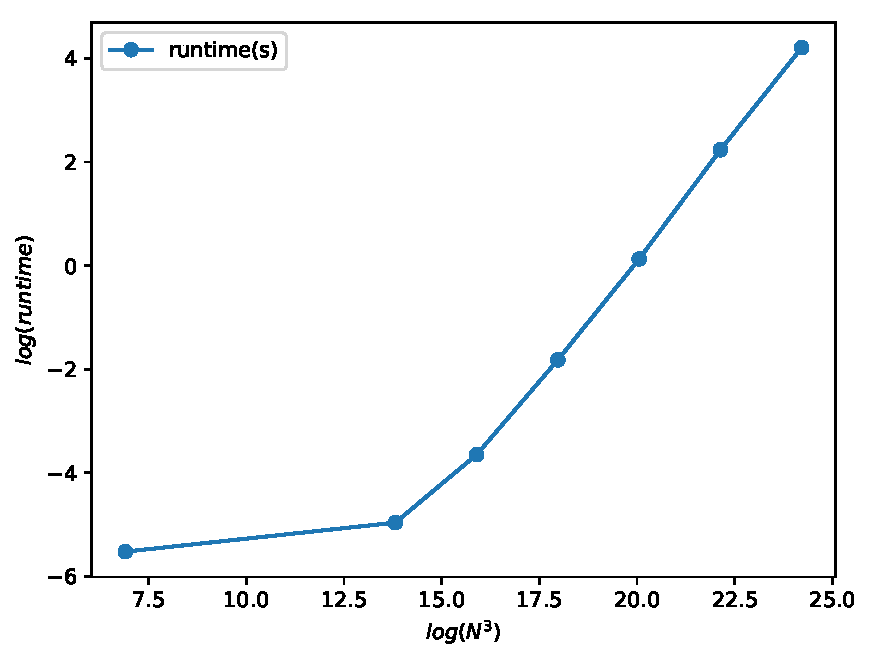
\includegraphics[width=0.65\textwidth]{src/runtime.pdf}
    \label{fig:runtime}
\end{figure}
\begin{figure}[H]
    \centering
    \caption{LU vs $N^3$}
    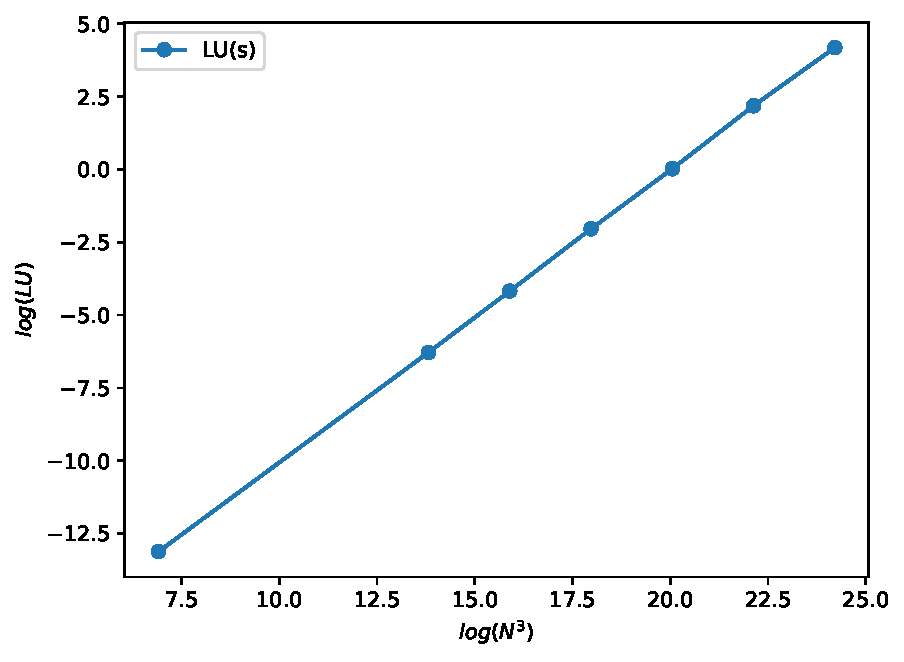
\includegraphics[width=0.65\textwidth]{src/LU.pdf}
    \label{fig:LU}
\end{figure}
\begin{figure}[H]
    \centering
    \caption{FWD vs $N^2$}
    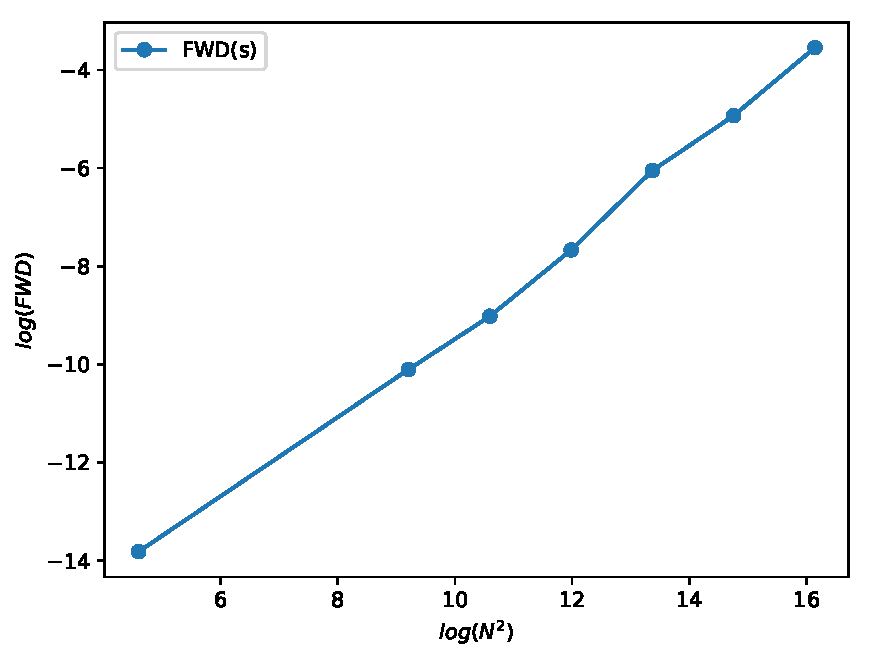
\includegraphics[width=0.65\textwidth]{src/FWD.pdf}
    \label{fig:fwd}
\end{figure}
\begin{figure}[H]
    \centering
    \caption{BCK vs $N^2$}
    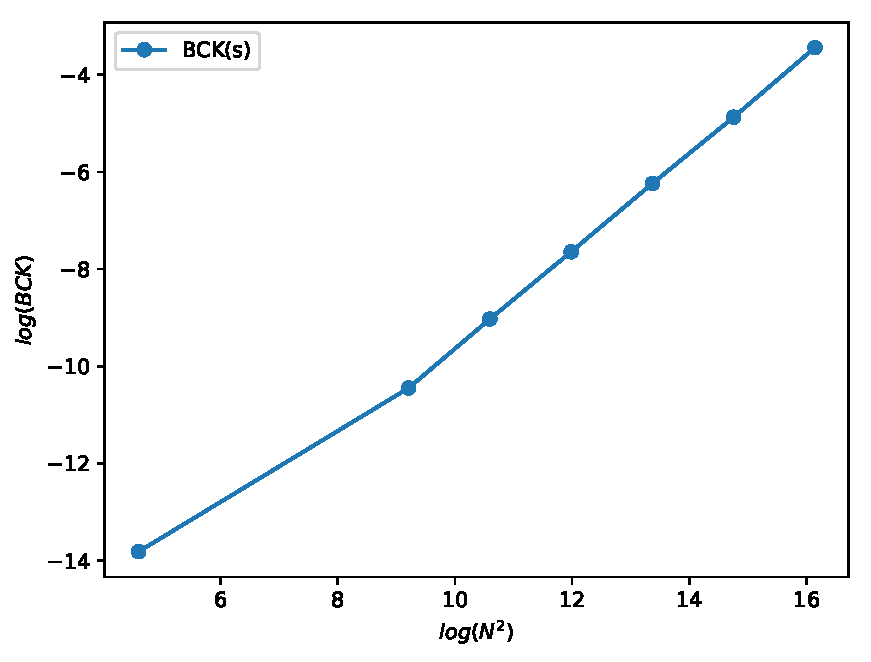
\includegraphics[width=0.65\textwidth]{src/BCK.pdf}
    \label{fig:bck}
\end{figure}

\end{document}










